\documentclass{article}\usepackage[]{graphicx}\usepackage[]{color}
%% maxwidth is the original width if it is less than linewidth
%% otherwise use linewidth (to make sure the graphics do not exceed the margin)
\makeatletter
\def\maxwidth{ %
  \ifdim\Gin@nat@width>\linewidth
    \linewidth
  \else
    \Gin@nat@width
  \fi
}
\makeatother

\definecolor{fgcolor}{rgb}{0.345, 0.345, 0.345}
\newcommand{\hlnum}[1]{\textcolor[rgb]{0.686,0.059,0.569}{#1}}%
\newcommand{\hlstr}[1]{\textcolor[rgb]{0.192,0.494,0.8}{#1}}%
\newcommand{\hlcom}[1]{\textcolor[rgb]{0.678,0.584,0.686}{\textit{#1}}}%
\newcommand{\hlopt}[1]{\textcolor[rgb]{0,0,0}{#1}}%
\newcommand{\hlstd}[1]{\textcolor[rgb]{0.345,0.345,0.345}{#1}}%
\newcommand{\hlkwa}[1]{\textcolor[rgb]{0.161,0.373,0.58}{\textbf{#1}}}%
\newcommand{\hlkwb}[1]{\textcolor[rgb]{0.69,0.353,0.396}{#1}}%
\newcommand{\hlkwc}[1]{\textcolor[rgb]{0.333,0.667,0.333}{#1}}%
\newcommand{\hlkwd}[1]{\textcolor[rgb]{0.737,0.353,0.396}{\textbf{#1}}}%

\usepackage{framed}
\makeatletter
\newenvironment{kframe}{%
 \def\at@end@of@kframe{}%
 \ifinner\ifhmode%
  \def\at@end@of@kframe{\end{minipage}}%
  \begin{minipage}{\columnwidth}%
 \fi\fi%
 \def\FrameCommand##1{\hskip\@totalleftmargin \hskip-\fboxsep
 \colorbox{shadecolor}{##1}\hskip-\fboxsep
     % There is no \\@totalrightmargin, so:
     \hskip-\linewidth \hskip-\@totalleftmargin \hskip\columnwidth}%
 \MakeFramed {\advance\hsize-\width
   \@totalleftmargin\z@ \linewidth\hsize
   \@setminipage}}%
 {\par\unskip\endMakeFramed%
 \at@end@of@kframe}
\makeatother

\definecolor{shadecolor}{rgb}{.97, .97, .97}
\definecolor{messagecolor}{rgb}{0, 0, 0}
\definecolor{warningcolor}{rgb}{1, 0, 1}
\definecolor{errorcolor}{rgb}{1, 0, 0}
\newenvironment{knitrout}{}{} % an empty environment to be redefined in TeX

\usepackage{alltt}

%\VignetteEngine{knitr::knitr}
%\VignetteIndexEntry{edge Package}


\usepackage{graphics}
\usepackage{amsmath}
\usepackage{fullpage}
\usepackage{bibentry}
\usepackage[section]{placeins}
\usepackage[round]{natbib}
\usepackage{authblk}
\usepackage[parfill]{parskip}
\setlength{\parskip}{10pt}
%\usepackage{indentfirst}
\usepackage[colorlinks=true]{hyperref}
\usepackage[utf8]{inputenc}
\nobibliography*
\IfFileExists{upquote.sty}{\usepackage{upquote}}{}
\begin{document}



\title{{\tt edge}:\\ Extraction of Differential Gene Expression \\ Version 0.99.0}

\author[1]{John D. Storey\thanks{\url{http://genomine.org/contact.html}}}
\author[2]{Jeffrey T. Leek}
\author[1]{Andrew J. Bass}
\affil[1]{Princeton University}
\affil[2]{John Hopkins University}

\renewcommand\Authands{ and }

\maketitle
\tableofcontents
\newpage
\section{Introduction}

{\tt edge} is a package for significance analysis of DNA micro-array experiments and is able to identify genes that are differentially expressed between two or more different biological conditions (e.g., healthy versus diseased tissue). {\tt edge} performs significance analysis by using a new method developed by \cite{storey:2007} called the optimal discovery procedure (ODP). Whereas previously existing methods employ statistics that are essentially designed for testing one gene at a time (e.g., t-statistics and F-statistics), the ODP-statistic uses information across all genes to test for differential expression. \cite{storey:etal:2007} shows that the ODP is a more intuitive, often times more powerful, approach to multiple hypothesis testing when compared to traditional methods. The improvements in power from using the optimal discovery procedure are substantial; Figure~\ref{fig:Comparison} shows a comparison between edge and five leading software packages based on the \cite{hedenfalk:2001} breast cancer expression study.

\texttt{edge} also implements strategies that have been specifically designed for time course experiments. Many things can go wrong when using methods that have been designed for static experiments, and even though some significance analysis packages allow for users to enter information about time points, \cite{storey:2005} developed a procedure that simplifies the modelling process for time course experiments. In addition to identifying differentially expressed genes in both static and time course studies, {\tt edge} includes implementations of popular packages such as {\tt snm}, {\tt sva} and {\tt qvalue} to help simplify the analysis process for researchers. 

The rest of the document details how to use {\tt edge} in three different case studies: static, independent time course and longitudinal time course. For additional information regarding the optimal discovery procedure or the \cite{storey:2005} methodology for time course experiments, see section~\ref{sec:citepackage}.

\section{Citing this package}
\label{sec:citepackage}
\textbf{[1] \bibentry{storey:2007}} \\
Theory paper that introduces the optimal discovery procedure and shows that it maximizes the expected true postive results for each number of fixed false positive results. The optimality is closely related to the false discovery rate.

\textbf{[2] \bibentry{storey:etal:2007}} \\
Dicusses various ways of estimating the ODP statistic with applications to microarray experiments.

\textbf{[3] \bibentry{woo:leek:storey:2011}} \\
Previous implementations of the ODP are computationally infeasible for a large number of hypothesis tests. This paper introduces a computationally efficient implementation of ODP that this package is based on.

\textbf{[4] \bibentry{storey:2005}} \\
A methodology for analyzing time course microarray data is introduced and applied to two time course studies on humans. 

\section{Getting help}
Hopefully, most questions relating to the package will be answered in the vignette but to get a more detailed account of how to use the functions simply type within R:
\begin{knitrout}
\definecolor{shadecolor}{rgb}{0.969, 0.969, 0.969}\color{fgcolor}\begin{kframe}
\begin{alltt}
\hlkwd{help}\hlstd{(}\hlkwc{package} \hlstd{=} \hlstr{"edge"}\hlstd{)}
\end{alltt}
\end{kframe}
\end{knitrout}
\noindent Please contact the authors directly with any issues regarding bugs. Otherwise, any questions or problems implementing {\tt edge} will most efficiently be addressed on the Bioconductor mailing list, \url{http://stat.ethz.ch/mailman/listinfo/bioconductor}.

\section{Quick start guide}
To get started, first load the {\tt kidney} dataset included in the package: 
\begin{knitrout}
\definecolor{shadecolor}{rgb}{0.969, 0.969, 0.969}\color{fgcolor}\begin{kframe}
\begin{alltt}
\hlkwd{library}\hlstd{(edge)}
\hlkwd{data}\hlstd{(kidney)}
\hlstd{kidexpr} \hlkwb{<-} \hlstd{kidney}\hlopt{$}\hlstd{kidexpr}
\hlstd{age} \hlkwb{<-} \hlstd{kidney}\hlopt{$}\hlstd{age}
\hlstd{sex} \hlkwb{<-} \hlstd{kidney}\hlopt{$}\hlstd{sex}
\end{alltt}
\end{kframe}
\end{knitrout}
The {\tt kidney} study is interested in determining differentially expressed genes in the kidney as it ages. The {\tt age} variable is the age of the subjects and the {\tt sex} variable is whether the subjects were male or female. The expression values for the genes are contained in the {\tt kidexpr} variable.

Once the data has been loaded, the user has two options to create an {\tt edgeSet} object: {\tt edgeModel} or {\tt edgeStudy}. If the experiment models are unknown to the user, {\tt edgeStudy} can be used to create the models:
\begin{knitrout}
\definecolor{shadecolor}{rgb}{0.969, 0.969, 0.969}\color{fgcolor}\begin{kframe}
\begin{alltt}
\hlstd{edgeObj} \hlkwb{<-} \hlkwd{edgeStudy}\hlstd{(}\hlkwc{data} \hlstd{= kidexpr,} \hlkwc{adj.var} \hlstd{= sex,}
    \hlkwc{tme} \hlstd{= age,} \hlkwc{sampling} \hlstd{=} \hlstr{"timecourse"}\hlstd{)}
\hlstd{fullMod} \hlkwb{<-} \hlkwd{fullModel}\hlstd{(edgeObj)}
\hlstd{nullMod} \hlkwb{<-} \hlkwd{nullModel}\hlstd{(edgeObj)}
\end{alltt}
\end{kframe}
\end{knitrout}
The variable {\tt sampling} describes the type of experiment performed, {\tt adj.var} is the adjustment variable and {\tt tme} is the time variable in the study. If the experiment is more complex then type {\tt ?edgeStudy} for additional arguments.  

If the alternative and null models are known to the user then {\tt edgeModel} can be used to make an {\tt edgeSet} object:
\begin{knitrout}
\definecolor{shadecolor}{rgb}{0.969, 0.969, 0.969}\color{fgcolor}\begin{kframe}
\begin{alltt}
\hlkwd{library}\hlstd{(splines)}
\hlcom{# alternative and null models}
\hlstd{cov} \hlkwb{<-} \hlkwd{data.frame}\hlstd{(}\hlkwc{sex} \hlstd{= sex,} \hlkwc{age} \hlstd{= age)}
\hlstd{null.model} \hlkwb{<-} \hlopt{~}\hlstd{sex}
\hlstd{full.model} \hlkwb{<-} \hlopt{~}\hlstd{sex} \hlopt{+} \hlkwd{ns}\hlstd{(age,} \hlkwc{df} \hlstd{=} \hlnum{4}\hlstd{)}

\hlstd{edgeObj} \hlkwb{<-} \hlkwd{edgeModel}\hlstd{(}\hlkwc{data} \hlstd{= kidexpr,} \hlkwc{cov} \hlstd{= cov,} \hlkwc{nullMod} \hlstd{= null.model,}
    \hlkwc{altMod} \hlstd{= full.model)}
\end{alltt}
\end{kframe}
\end{knitrout}
The {\tt cov} is a data frame of covariates, the {\tt nullMod} is the null model and the {\tt altMod} is the alternative model. The input {\tt cov} is a data frame with the column names the same as the variables in the alternative and null models. See \cite{storey:2005} to see why a natural spline curve is fit to the time variable in the study. 

The {\tt odp} or {\tt lrt} function can be used on {\tt edgeObj} to implement either the optimal discovery procedure or the likelihood ratio test, respectively:
\begin{knitrout}
\definecolor{shadecolor}{rgb}{0.969, 0.969, 0.969}\color{fgcolor}\begin{kframe}
\begin{alltt}
\hlcom{# optimal discovery procedure}
\hlstd{edgeODP} \hlkwb{<-} \hlkwd{odp}\hlstd{(edgeObj,} \hlkwc{verbose} \hlstd{=} \hlnum{FALSE}\hlstd{)}
\hlcom{# likelihood ratio test}
\hlstd{edgeLRT} \hlkwb{<-} \hlkwd{lrt}\hlstd{(edgeObj)}
\end{alltt}
\end{kframe}
\end{knitrout}
To access the p-values, q-values and local false discovery rates for each gene, use the function {\tt qvalueObj}:
\begin{knitrout}
\definecolor{shadecolor}{rgb}{0.969, 0.969, 0.969}\color{fgcolor}\begin{kframe}
\begin{alltt}
\hlstd{qvalObj} \hlkwb{<-} \hlkwd{qvalueObj}\hlstd{(edgeODP)}
\hlstd{qvals} \hlkwb{<-} \hlstd{qvalObj}\hlopt{$}\hlstd{qvalues}
\hlstd{pvals} \hlkwb{<-} \hlstd{qvalObj}\hlopt{$}\hlstd{pvalues}
\hlstd{lfdr} \hlkwb{<-} \hlstd{qvalObj}\hlopt{$}\hlstd{lfdr}
\hlstd{pi0} \hlkwb{<-} \hlstd{qvalObj}\hlopt{$}\hlstd{pi0}
\end{alltt}
\end{kframe}
\end{knitrout}
The following sections of the manual go through various case studies for a more comprehensive overview of the {\tt edge} package.

\section{Case study: static experiment}
\label{sec:gibson}
In the static sampling experiment, the arrays have been collected from distinct biological groups without respect to time. The goal is to identify genes that have a statistically significant difference in average expression across these distinct biological groups. 

The {\tt gibson} dataset provides gene expression measurements in peripheral blood leukocyte samples from three Moroccan Amazigh groups leading distinct ways of life: desert nomadic (DESERT), mountain agrarian (VILLAGE), and coastal urban (AGADIR). We are interested in finding the genes that differentiate the Moroccan Amazigh groups the most. See \cite{gibson:2008} for additional information regarding the data.

\subsection{Importing the data}
To import the {\tt gibson} data use the {\tt data} function:
\begin{knitrout}
\definecolor{shadecolor}{rgb}{0.969, 0.969, 0.969}\color{fgcolor}\begin{kframe}
\begin{alltt}
\hlkwd{data}\hlstd{(gibson)}
\hlkwd{names}\hlstd{(gibson)}
\end{alltt}
\begin{verbatim}
## [1] "gender"   "location" "batch"    "gibexpr"
\end{verbatim}
\end{kframe}
\end{knitrout}
There are a few variables in the data set: {\tt batch}, {\tt gibexpr}, {\tt gender}, and {\tt location}. The three covariates of interest are {\tt gender}, {\tt batch} and {\tt location}. The biological variable is the {\tt location} variable, which contains information on where individuals are sampled: ``VILLAGE'', ``DESERT'' or ``AGADIR''. The {\tt gender} variable specifies whether the individual is a male or a female and there are two different {\tt batches} in the study. The {\tt gibexpr} variable contains the gene expression measurements. 

As an example, the expression values of the first gene are shown in Figure~\ref{fig:gplot}. In the figure, it appears that that individuals from ``VILLAGE'' are less expressed when compared to other lifestyles. We should stop short of that observation because the data needs to be adjusted with the experimental models. Before that, the alternative and null model of the study needs to be formulated which is discussed the next section.

\subsection{Creating the alternative and null models}
In order to find differentially expressed genes, there first needs to be an alternative and null model for the study. There are two ways to input the experimental models in {\tt edge}: {\tt edgeModel} and {\tt edgeStudy}. {\tt edgeStudy} should be used by users unfamiliar with formulating the alternative and null models but are familiar with the covariates in the study: 
\begin{knitrout}
\definecolor{shadecolor}{rgb}{0.969, 0.969, 0.969}\color{fgcolor}\begin{kframe}
\begin{alltt}
\hlstd{edgeObj} \hlkwb{<-} \hlkwd{edgeStudy}\hlstd{(}\hlkwc{data} \hlstd{= gibson}\hlopt{$}\hlstd{gibexpr,} \hlkwc{adj.var} \hlstd{=} \hlkwd{cbind}\hlstd{(gibson}\hlopt{$}\hlstd{gender,}
    \hlstd{gibson}\hlopt{$}\hlstd{batch),} \hlkwc{grp} \hlstd{= gibson}\hlopt{$}\hlstd{location,} \hlkwc{sampling} \hlstd{=} \hlstr{"static"}\hlstd{)}
\end{alltt}
\end{kframe}
\end{knitrout}

{\tt adj.var} is for the adjustment variables, {\tt grp} is the variable containing the group assignments for each individual in the study and {\tt sampling} describes the type of experiment. Since {\tt gibson} is a static study, the {\tt sampling} argument will be ``static''. The {\tt grp} variable will be the {\tt location} variable and the adjustment variables are {\tt gender} and {\tt batch}.

Alternatively, if the user is familiar with their alternative and null models in the study then {\tt edgeModel} can be used to input the models directly:
\begin{knitrout}
\definecolor{shadecolor}{rgb}{0.969, 0.969, 0.969}\color{fgcolor}\begin{kframe}
\begin{alltt}
\hlstd{cov} \hlkwb{<-} \hlkwd{data.frame}\hlstd{(}\hlkwc{Gender} \hlstd{= gibson}\hlopt{$}\hlstd{gender,} \hlkwc{Batch} \hlstd{= gibson}\hlopt{$}\hlstd{batch,}
    \hlkwc{Location} \hlstd{= gibson}\hlopt{$}\hlstd{location)}
\hlstd{null.model} \hlkwb{<-} \hlopt{~}\hlstd{Gender} \hlopt{+} \hlstd{Batch}
\hlstd{alt.model} \hlkwb{<-} \hlopt{~}\hlstd{Gender} \hlopt{+} \hlstd{Batch} \hlopt{+} \hlstd{Location}
\hlstd{edgeObj} \hlkwb{<-} \hlkwd{edgeModel}\hlstd{(}\hlkwc{data} \hlstd{= gibson}\hlopt{$}\hlstd{gibexpr,} \hlkwc{cov} \hlstd{= cov,}
    \hlkwc{altMod} \hlstd{= alt.model,} \hlkwc{nullMod} \hlstd{= null.model)}
\end{alltt}
\end{kframe}
\end{knitrout}

The {\tt cov} argument is a data frame of all the relevant covariates, {\tt altMod} and {\tt nullMod} are the alternative and null models of the experiment, respectively. Notice that the models must be formatted as a formula and contain the same variable names as in the {\tt cov} data frame. The null model contains the {\tt gender} and {\tt batch} covariates and the alternative model includes the {\tt location} variable. Therefore, we are interested in testing whether the alternative model improves the model fit of a gene significantly when compared to the null model. If it does not, then we can conclude that there is no significant difference between Moroccan Amazigh groups for this particular gene. 

The variable {\tt edgeObj} is an {\tt edgeSet} object that stores all the relevant experimental data. The {\tt edgeSet} object is discussed further in the next section. 

\subsection{The {\tt edgeSet} object}
Once either {\tt edgeModel} or {\tt edgeStudy} is used, an {\tt edgeSet} object is created. To view the slots contained in the object:
\begin{knitrout}
\definecolor{shadecolor}{rgb}{0.969, 0.969, 0.969}\color{fgcolor}\begin{kframe}
\begin{alltt}
\hlkwd{slotNames}\hlstd{(edgeObj)}
\end{alltt}
\begin{verbatim}
##  [1] "null.model"        "full.model"       
##  [3] "null.matrix"       "full.matrix"      
##  [5] "individual"        "qvalueObj"        
##  [7] "experimentData"    "assayData"        
##  [9] "phenoData"         "featureData"      
## [11] "annotation"        "protocolData"     
## [13] ".__classVersion__"
\end{verbatim}
\end{kframe}
\end{knitrout}
A description of each slot is listed below: 
\begin{itemize}
\item {\tt full.model}: the alternative model of the experiment
\item {\tt null.model}: the null model of the experiment
\item {\tt full.matrix}: the alternative model in matrix form
\item {\tt null.matrix}: the null model in matrix form
\item {\tt individual}: variable that keeps track of individuals (same individuals are sampled multiple times)
\item {\tt qvalueObj}: {\tt qvalue} list. Contains p-values, q-values and local false discovery rates of the significance analysis. See the {\tt qvalue} package for more details.
\item {\tt ExpressionSet}: inherits the slots from {\tt ExpressionSet} object
\end{itemize}

{\tt ExpressionSet} contains the expression measurements and other information from the experiment. The {\tt edgeSet} object inherits all the functions from an {\tt ExpressionSet} object. As an example, to access the expression values, one can use the function {\tt exprs} or to access the covariates, {\tt pData}:
\begin{knitrout}
\definecolor{shadecolor}{rgb}{0.969, 0.969, 0.969}\color{fgcolor}\begin{kframe}
\begin{alltt}
\hlstd{gibexpr} \hlkwb{<-} \hlkwd{exprs}\hlstd{(edgeObj)}
\hlstd{cov} \hlkwb{<-} \hlkwd{pData}\hlstd{(edgeObj)}
\end{alltt}
\end{kframe}
\end{knitrout}
The {\tt ExpressionSet} class is a widely used object in Bioconductor and more information can be found \url{http://www.bioconductor.org/packages/2.14/bioc/html/Biobase.html}. See the advanced section to get a better understanding of how {\tt ExpressionSet} objects integrate into the {\tt edge} framework.

As an example of how to access the slots of {\tt edgeObj} suppose we are interested in viewing the alternative and null models. The models can be accessed by:
\begin{knitrout}
\definecolor{shadecolor}{rgb}{0.969, 0.969, 0.969}\color{fgcolor}\begin{kframe}
\begin{alltt}
\hlkwd{fullModel}\hlstd{(edgeObj)}
\end{alltt}
\begin{verbatim}
## ~Gender + Batch + Location
\end{verbatim}
\begin{alltt}
\hlkwd{nullModel}\hlstd{(edgeObj)}
\end{alltt}
\begin{verbatim}
## ~Gender + Batch
\end{verbatim}
\end{kframe}
\end{knitrout}
Next, we can extract the models in matrix form for computational analysis:
\begin{knitrout}
\definecolor{shadecolor}{rgb}{0.969, 0.969, 0.969}\color{fgcolor}\begin{kframe}
\begin{alltt}
\hlstd{full.matrix} \hlkwb{<-} \hlkwd{fullMatrix}\hlstd{(edgeObj)}
\hlstd{null.matrix} \hlkwb{<-} \hlkwd{nullMatrix}\hlstd{(edgeObj)}
\end{alltt}
\end{kframe}
\end{knitrout}
See {\tt ?edgeSet} for additional functions to access different slots of the {\tt edgeSet} object. 

\subsection{Fitting the data}
The {\tt edgeFit} function is an implementation of least squares using the alternative and null models:
\begin{knitrout}
\definecolor{shadecolor}{rgb}{0.969, 0.969, 0.969}\color{fgcolor}\begin{kframe}
\begin{alltt}
\hlstd{efObj} \hlkwb{<-} \hlkwd{edgeFit}\hlstd{(edgeObj,} \hlkwc{stat.type} \hlstd{=} \hlstr{"lrt"}\hlstd{)}
\end{alltt}
\end{kframe}
\end{knitrout}
The {\tt stat.type} argument specifies whether you want the {\tt odp} or {\tt lrt} fitted values. The difference between choosing ``odp'' and ``lrt'' is that ``odp'' centers the data by the null model fit which is necessary for downstream analysis in the optimal discovery procedure. {\tt edgeFit} creates another object with the following slots:
\begin{itemize}
\item {\tt fit.full}: fitted values from the alternative model
\item {\tt fit.null}: fitted values from null model
\item {\tt res.full}: residuals from the alternative model
\item {\tt res.null}: residuals from the null model
\item {\tt dH.full}: diagonal elements in the projection matrix for the full model
\item {\tt beta.coef}: the coefficients for the full model
\item {\tt stat.type}: statistic type used, either ``odp'' or ``lrt''
\end{itemize}

To access the fitted coefficients of the alternative model in {\tt efObj}:
\begin{knitrout}
\definecolor{shadecolor}{rgb}{0.969, 0.969, 0.969}\color{fgcolor}\begin{kframe}
\begin{alltt}
\hlkwd{betaCoef}\hlstd{(efObj)}
\end{alltt}
\end{kframe}
\end{knitrout}
To access the alternative and null residuals:
\begin{knitrout}
\definecolor{shadecolor}{rgb}{0.969, 0.969, 0.969}\color{fgcolor}\begin{kframe}
\begin{alltt}
\hlstd{alt.res} \hlkwb{<-} \hlkwd{resFull}\hlstd{(efObj)}
\hlstd{null.res} \hlkwb{<-} \hlkwd{resNull}\hlstd{(efObj)}
\end{alltt}
\end{kframe}
\end{knitrout}
To access the fitted values:
\begin{knitrout}
\definecolor{shadecolor}{rgb}{0.969, 0.969, 0.969}\color{fgcolor}\begin{kframe}
\begin{alltt}
\hlstd{alt.fitted} \hlkwb{<-} \hlkwd{fitFull}\hlstd{(efObj)}
\hlstd{null.fitted} \hlkwb{<-} \hlkwd{fitNull}\hlstd{(efObj)}
\end{alltt}
\end{kframe}
\end{knitrout}

See {\tt ?edgeFit} for more details on accessing the slots in an {\tt edgeFit} object. The fitted values of the first gene is shown in Figure~\ref{fig:gplotFit}. The null model fit is the average expression value across the interaction of {\tt batch} and {\tt sex}. The alternative model fit seems to pick up some differences relative to the null model. Next, we have to test whether the observed differences between models in Figure~\ref{fig:gplotFit} is significant.

\subsection{Significance analysis}
Interpreting the models in a hypothesis test is very intuitive: Does the alternative model better fit the data when compared to the null model? For the fitted values of the first gene plotted in Figure~\ref{fig:gplotFit}, it seems that the alternative model fits the data better than the null model. In order to conclude it's significant, we need to calculate the p-value. The user can use either the optimal discovery procedure or likelihood ratio test. 

\subsubsection{Likelihood ratio test}
The {\tt lrt} function performs a likelihood ratio test to determine p-values:
\begin{knitrout}
\definecolor{shadecolor}{rgb}{0.969, 0.969, 0.969}\color{fgcolor}\begin{kframe}
\begin{alltt}
\hlstd{edgeLRT} \hlkwb{<-} \hlkwd{lrt}\hlstd{(edgeObj,} \hlkwc{nullDistn} \hlstd{=} \hlstr{"normal"}\hlstd{)}
\end{alltt}
\end{kframe}
\end{knitrout}
If the null distribution, {\tt nullDistn}, is calculated using ``bootstrap'' then residuals from the alternative model are re-sampled and added to the null model to simulate a distribution where there is no differential expression. Otherwise, the default input is ``normal'' and the assumption is that the null statistics follow a F-distribution. See {\tt lrt} for additional arguments.



\subsubsection{Optimal discovery procedure}
{\tt odp} performs the optimal discovery procedure, which is a new approach for optimally performing many hypothesis tests in a high-dimensional study. When testing a feature, information from all the features is utilized when testing for significance of a feature. It guarentees to maximize the number of expected true positive results for each fixed number of expected false positive results which is related to FDR. The optimal discovery procedure can be implemented on an {\tt edgeSet} object by the {\tt odp} function:
\begin{knitrout}
\definecolor{shadecolor}{rgb}{0.969, 0.969, 0.969}\color{fgcolor}\begin{kframe}
\begin{alltt}
\hlstd{edgeODP} \hlkwb{<-} \hlkwd{odp}\hlstd{(edgeObj,} \hlkwc{bs.its} \hlstd{=} \hlnum{30}\hlstd{,} \hlkwc{verbose} \hlstd{=} \hlnum{FALSE}\hlstd{,}
    \hlkwc{n.mods} \hlstd{=} \hlnum{50}\hlstd{)}
\end{alltt}
\end{kframe}
\end{knitrout}
The number of bootstrap iterations is controlled by {\tt bs.its}, {\tt verbose} prints each bootstrap iteration number and {\tt n.mods} is the number of clusters. 

{\tt n.mods} controls the number of clusters in the k-means algorithm where genes are assigned to a cluster based on the Kullback-Leiber distance. If {\tt n.mods} is equal to the number of genes then the original optimal discovery procedure is used. Depending on the number of genes, this setting can take a very long time.  Therefore, it is recommended to use a small {\tt n.mods} value to substantially decrease the computational time. In \cite{woo:leek:storey:2011}, it is shown that assigning {\tt n.mods} to about 50 will cause a negligible loss in power. Type {\tt ?odp} for more details on the algorithm. The number of {\tt bs.its} iterations recommended is 100.

\subsection{Significance results}
The {\tt summary} function can be used on an {\tt edgeSet} object to give an overview of the analysis:
\begin{knitrout}
\definecolor{shadecolor}{rgb}{0.969, 0.969, 0.969}\color{fgcolor}\begin{kframe}
\begin{alltt}
\hlkwd{summary}\hlstd{(edgeODP)}
\end{alltt}
\begin{verbatim}
## 
## ExpressionSet Summary 
##  
## ExpressionSet (storageMode: lockedEnvironment)
## assayData: 10177 features, 46 samples 
##   element names: exprs 
## protocolData: none
## phenoData
##   sampleNames: 1 2 ... 46 (46 total)
##   varLabels: Gender Batch Location
##   varMetadata: labelDescription
## featureData: none
## experimentData: use 'experimentData(object)'
## Annotation:  
## 
## edge Analysis Summary 
##  
## Total number of arrays: 46 
## Total number of probes: 10177 
##  
## Biological variables: 
## 	Null Model:~Gender + Batch
## 
## 	Full Model:~Gender + Batch + Location
## 
## ....... 
##  
## 
## Statistical significance summary:
## pi0:	0.2991622	
## 
## Cumulative number of significant calls:
## 
##           <1e-04 <0.001 <0.01 <0.025 <0.05 <0.1
## p-value      932   1679  2934   3783  4571 5487
## q-value      744   1362  2903   4117  5251 6863
## local fdr    492    847  1869   2500  3185 4194
##              <1
## p-value   10177
## q-value   10177
## local fdr  9530
\end{verbatim}
\end{kframe}
\end{knitrout}
There are three core summaries: {\tt ExpressionSet} summary, {\tt edge} analysis and statistical significance summary. The {\tt ExpressionSet} summary shows a summary of the {\tt ExpressionSet} object. {\tt edge} analysis shows an overview of the models used and other information about the dataset. The significance analysis shows the proportion of null genes, $\pi_{0}$, and significant genes at various cutoffs in terms of p-values, q-values and local false discovery rates.

The function {\tt qvalueObj} can be used on {\tt edgeODP} to extract the significance results:
\begin{knitrout}
\definecolor{shadecolor}{rgb}{0.969, 0.969, 0.969}\color{fgcolor}\begin{kframe}
\begin{alltt}
\hlstd{sig.results} \hlkwb{<-} \hlkwd{qvalueObj}\hlstd{(edgeODP)}
\end{alltt}
\end{kframe}
\end{knitrout}

The object {\tt sig.results} is a list with the following slots:
\begin{knitrout}
\definecolor{shadecolor}{rgb}{0.969, 0.969, 0.969}\color{fgcolor}\begin{kframe}
\begin{alltt}
\hlkwd{names}\hlstd{(sig.results)}
\end{alltt}
\begin{verbatim}
## [1] "call"       "pi0"        "qvalues"   
## [4] "pvalues"    "lfdr"       "pi0.lambda"
## [7] "lambda"     "pi0.smooth"
\end{verbatim}
\end{kframe}
\end{knitrout}
The key variables are {\tt pi0}, {\tt pvalues}, {\tt lfdr} and {\tt qvalues}. The {\tt pi0} variable provides an estimate of the proportion of null p-values, {\tt pvalues} are the p-values, {\tt qvalues} are the estimated q-values and {\tt lfdr} are the local false discovery rates. Using the function {\tt hist} on {\tt sig.results} will produce a p-value histogram along with the density curves of q-values and local false discovery rate values. See Figure~\ref{fig:gqvalHist}.

The q-value controls the false discovery at a level {\tt alpha} and so making significance decisions with q-values is recommended. Q-values measure the proportion of false positives incurred when calling a particular test significant. For example, to complete our analysis of gene 1 in this example, lets view the q-value estimate:
\begin{knitrout}
\definecolor{shadecolor}{rgb}{0.969, 0.969, 0.969}\color{fgcolor}\begin{kframe}
\begin{alltt}
\hlstd{qval} \hlkwb{<-} \hlstd{sig.results}\hlopt{$}\hlstd{qvalues}
\hlstd{qval[}\hlnum{1}\hlstd{]}
\end{alltt}
\begin{verbatim}
## [1] 3.659477e-05
\end{verbatim}
\end{kframe}
\end{knitrout}

So at this particular gene, the q-value is $3.6e-5$. If we consider a false discovery cutoff rate of 0.01 then this gene is highly significant. Therefore, the observed differences observed in Figure~\ref{fig:gplotFit} are indeed significant so this particular gene is differentially expressed at each location. 

To get a list of all the signifcant genes at a false discovery rate cutoff of 0.01:
\begin{knitrout}
\definecolor{shadecolor}{rgb}{0.969, 0.969, 0.969}\color{fgcolor}\begin{kframe}
\begin{alltt}
\hlstd{fdr.level} \hlkwb{<-} \hlnum{0.01}
\hlstd{sigGenes} \hlkwb{<-} \hlstd{qval} \hlopt{<} \hlstd{fdr.level}
\end{alltt}
\end{kframe}
\end{knitrout}

\section{Case study: independent time course experiment}
\label{sec:kidney}
In the independent time course study, the arrays have been sampled with respect to time from one biological group and the goal is to identify genes that show ``within-class temporal differential expression'', i.e., genes that show statistically significant changes in expression over time.

Gene expression measurements from {\tt kidney} samples were obtained from 72 human subjects ranging in age from 27 to 92 years. Only one array was obtained per sample and the age and tissue type of each subject was recorded. See \cite{rodwell:2004} for additional information regarding the dataset.

\subsection{Importing the data}
To import the {\tt kidney} data use the {\tt data} function:
\begin{knitrout}
\definecolor{shadecolor}{rgb}{0.969, 0.969, 0.969}\color{fgcolor}\begin{kframe}
\begin{alltt}
\hlkwd{data}\hlstd{(kidney)}
\hlkwd{names}\hlstd{(kidney)}
\end{alltt}
\begin{verbatim}
## [1] "tissue"  "age"     "sex"     "kidexpr"
\end{verbatim}
\end{kframe}
\end{knitrout}

There are a few covariates in this data set: {\tt sex}, {\tt age}, {\tt tissue}, {\tt kidexpr} and {\tt kidcov}. We will focus on the expression values of the cortex {\tt tissue} samples:
\begin{knitrout}
\definecolor{shadecolor}{rgb}{0.969, 0.969, 0.969}\color{fgcolor}\begin{kframe}
\begin{alltt}
\hlstd{sex} \hlkwb{<-} \hlstd{kidney}\hlopt{$}\hlstd{sex[kidney}\hlopt{$}\hlstd{tissue} \hlopt{==} \hlstr{"c"}\hlstd{]}
\hlstd{age} \hlkwb{<-} \hlstd{kidney}\hlopt{$}\hlstd{age[kidney}\hlopt{$}\hlstd{tissue} \hlopt{==} \hlstr{"c"}\hlstd{]}
\hlstd{kidexpr} \hlkwb{<-} \hlkwd{log}\hlstd{(kidney}\hlopt{$}\hlstd{kidexpr[, kidney}\hlopt{$}\hlstd{tissue} \hlopt{==}
    \hlstr{"c"}\hlstd{]} \hlopt{+} \hlnum{10}\hlstd{)}
\end{alltt}
\end{kframe}
\end{knitrout}

The two main covariates of interest for this example are the {\tt sex} and {\tt age} covariates. The {\tt sex} variable is whether the subject was male or female and the {\tt age} variable is the age of the patients. {\tt kidexpr} contains the gene expression values for the study.

As an example, the expression values of the first gene are shown in Figure~\ref{fig:kplot}. It is very difficult to find a trend for this particular gene. Instead, we need to adjust the data with the models in the study. 

\subsection{Creating the alternative and null models}
In order to find differentially expressed genes, there first needs to be an alternative and null model for the study. There are two ways to input the experimental models in {\tt edge}: {\tt edgeModel} and {\tt edgeStudy}. {\tt edgeStudy} should be used by users unfamiliar with formulating the alternative and null models but are familiar with the covariates in the study: 
\begin{knitrout}
\definecolor{shadecolor}{rgb}{0.969, 0.969, 0.969}\color{fgcolor}\begin{kframe}
\begin{alltt}
\hlstd{edgeObj} \hlkwb{<-} \hlkwd{edgeStudy}\hlstd{(}\hlkwc{data} \hlstd{= kidexpr,} \hlkwc{adj.var} \hlstd{= sex,}
    \hlkwc{bio.var} \hlstd{= age,} \hlkwc{sampling} \hlstd{=} \hlstr{"timecourse"}\hlstd{)}
\end{alltt}
\end{kframe}
\end{knitrout}

{\tt adj.var} is for the adjustment variables, {\tt bio.var} is the biological variable and {\tt sampling} describes the type of experiment. Since {\tt kidney} is a time course study, the {\tt sampling} argument will be ``timecourse''. The {\tt bio.var} variable will be the {\tt age} variable and the adjustment variable is {\tt sex}.

Alternatively, if the user is familiar with their alternative and null models in the study then {\tt edgeModel} can be used to input the models directly:
\begin{knitrout}
\definecolor{shadecolor}{rgb}{0.969, 0.969, 0.969}\color{fgcolor}\begin{kframe}
\begin{alltt}
\hlstd{cov} \hlkwb{<-} \hlkwd{data.frame}\hlstd{(}\hlkwc{sex} \hlstd{= sex,} \hlkwc{age} \hlstd{= age)}
\hlstd{null.model} \hlkwb{<-} \hlopt{~}\hlstd{sex}
\hlstd{alt.model} \hlkwb{<-} \hlopt{~}\hlstd{sex} \hlopt{+} \hlkwd{ns}\hlstd{(age,} \hlkwc{df} \hlstd{=} \hlnum{4}\hlstd{)}
\hlstd{edgeKid} \hlkwb{<-} \hlkwd{edgeModel}\hlstd{(}\hlkwc{data} \hlstd{= kidexpr,} \hlkwc{cov} \hlstd{= cov,} \hlkwc{altMod} \hlstd{= alt.model,}
    \hlkwc{nullMod} \hlstd{= null.model)}
\end{alltt}


{\ttfamily\noindent\bfseries\color{errorcolor}{\#\# Error in eval(expr, envir, enclos): could not find function "{}ns"{}}}\end{kframe}
\end{knitrout}

The {\tt cov} argument is a data frame of all the relevant covariates, {\tt altMod} and {\tt nullMod} are the alternative and null models of the experiment, respectively. Notice that the models must be formatted as a formula and contain the same variable names as in the {\tt cov} data frame. The null model contains the {\tt sex} covariate and the alternative model includes the {\tt age} variable. Therefore, we are interested in testing whether the alternative model improves the model fit of a gene significantly when compared to the null model. If it does not, then we can conclude that there is no significant difference in this gene as it ages in the kidney. 

The variable {\tt edgeObj} is an {\tt edgeSet} object that stores all the relevant experimental data. The {\tt edgeSet} object is discussed further in the next section. 

\subsection{The {\tt edgeSet} object}
Once either {\tt edgeModel} or {\tt edgeStudy} is used, an {\tt edgeSet} object is created. To view the slots contained in the object:
\begin{knitrout}
\definecolor{shadecolor}{rgb}{0.969, 0.969, 0.969}\color{fgcolor}\begin{kframe}
\begin{alltt}
\hlkwd{slotNames}\hlstd{(edgeObj)}
\end{alltt}
\begin{verbatim}
##  [1] "null.model"        "full.model"       
##  [3] "null.matrix"       "full.matrix"      
##  [5] "individual"        "qvalueObj"        
##  [7] "experimentData"    "assayData"        
##  [9] "phenoData"         "featureData"      
## [11] "annotation"        "protocolData"     
## [13] ".__classVersion__"
\end{verbatim}
\end{kframe}
\end{knitrout}
A description of each slot is listed below: 
\begin{itemize}
\item {\tt full.model}: the alternative model of the experiment
\item {\tt null.model}: the null model of the experiment
\item {\tt full.matrix}: the alternative model in matrix form
\item {\tt null.matrix}: the null model in matrix form
\item {\tt individual}: variable that keeps track of individuals (same individuals are sampled multiple times)
\item {\tt qvalueObj}: {\tt qvalue} list. Contains p-values, q-values and local false discovery rates of the significance analysis. See the {\tt qvalue} package for more details.
\item {\tt ExpressionSet}: inherits the slots from {\tt ExpressionSet} object
\end{itemize}

{\tt ExpressionSet} contains the expression measurements and other information from the experiment. The {\tt edgeSet} object inherits all the functions from an {\tt ExpressionSet} object. As an example, to access the expression values, one can use the function {\tt exprs} or to access the covariates, {\tt pData}:
\begin{knitrout}
\definecolor{shadecolor}{rgb}{0.969, 0.969, 0.969}\color{fgcolor}\begin{kframe}
\begin{alltt}
\hlstd{gibexpr} \hlkwb{<-} \hlkwd{exprs}\hlstd{(edgeObj)}
\hlstd{cov} \hlkwb{<-} \hlkwd{pData}\hlstd{(edgeObj)}
\end{alltt}
\end{kframe}
\end{knitrout}
The {\tt ExpressionSet} class is a widely used object in Bioconductor and more information can be found \url{http://www.bioconductor.org/packages/2.14/bioc/html/Biobase.html}. See the advanced section to get a better understanding of how {\tt ExpressionSet} objects integrate into the {\tt edge} framework.

As an example of how to access the slots of {\tt edgeObj} suppose we are interested in viewing the alternative and null models. The models can be accessed by:
\begin{knitrout}
\definecolor{shadecolor}{rgb}{0.969, 0.969, 0.969}\color{fgcolor}\begin{kframe}
\begin{alltt}
\hlkwd{fullModel}\hlstd{(edgeObj)}
\end{alltt}
\begin{verbatim}
## ~adj.var + bio.var
## <environment: 0x10e229c8>
\end{verbatim}
\begin{alltt}
\hlkwd{nullModel}\hlstd{(edgeObj)}
\end{alltt}
\begin{verbatim}
## ~adj.var
## <environment: 0x10e229c8>
\end{verbatim}
\end{kframe}
\end{knitrout}
Next, we can extract the models in matrix form for computational analysis:
\begin{knitrout}
\definecolor{shadecolor}{rgb}{0.969, 0.969, 0.969}\color{fgcolor}\begin{kframe}
\begin{alltt}
\hlstd{full.matrix} \hlkwb{<-} \hlkwd{fullMatrix}\hlstd{(edgeObj)}
\hlstd{null.matrix} \hlkwb{<-} \hlkwd{nullMatrix}\hlstd{(edgeObj)}
\end{alltt}
\end{kframe}
\end{knitrout}
See {\tt ?edgeSet} for additional functions to access different slots of the {\tt edgeSet} object. 

\subsection{Fitting the data}
The {\tt edgeFit} function is an implementation of least squares using the alternative and null models:
\begin{knitrout}
\definecolor{shadecolor}{rgb}{0.969, 0.969, 0.969}\color{fgcolor}\begin{kframe}
\begin{alltt}
\hlstd{efObj} \hlkwb{<-} \hlkwd{edgeFit}\hlstd{(edgeObj,} \hlkwc{stat.type} \hlstd{=} \hlstr{"lrt"}\hlstd{)}
\end{alltt}
\end{kframe}
\end{knitrout}
The {\tt stat.type} argument specifies whether you want the {\tt odp} or {\tt lrt} fitted values. The difference between choosing ``odp'' and ``lrt'' is that ``odp'' centers the data by the null model fit which is necessary for downstream analysis in the optimal discovery procedure. {\tt edgeFit} creates another object with the following slots:
\begin{itemize}
\item {\tt fit.full}: fitted values from the alternative model
\item {\tt fit.null}: fitted values from null model
\item {\tt res.full}: residuals from the alternative model
\item {\tt res.null}: residuals from the null model
\item {\tt dH.full}: diagonal elements in the projection matrix for the full model
\item {\tt beta.coef}: the coefficients for the full model
\item {\tt stat.type}: statistic type used, either ``odp'' or ``lrt''
\end{itemize}

To access the fitted coefficients of the alternative model in {\tt efObj}:
\begin{knitrout}
\definecolor{shadecolor}{rgb}{0.969, 0.969, 0.969}\color{fgcolor}\begin{kframe}
\begin{alltt}
\hlkwd{betaCoef}\hlstd{(efObj)}
\end{alltt}
\end{kframe}
\end{knitrout}
To access the alternative and null residuals:
\begin{knitrout}
\definecolor{shadecolor}{rgb}{0.969, 0.969, 0.969}\color{fgcolor}\begin{kframe}
\begin{alltt}
\hlstd{alt.res} \hlkwb{<-} \hlkwd{resFull}\hlstd{(efObj)}
\hlstd{null.res} \hlkwb{<-} \hlkwd{resNull}\hlstd{(efObj)}
\end{alltt}
\end{kframe}
\end{knitrout}
To access the fitted values:
\begin{knitrout}
\definecolor{shadecolor}{rgb}{0.969, 0.969, 0.969}\color{fgcolor}\begin{kframe}
\begin{alltt}
\hlstd{alt.fitted} \hlkwb{<-} \hlkwd{fitFull}\hlstd{(efObj)}
\hlstd{null.fitted} \hlkwb{<-} \hlkwd{fitNull}\hlstd{(efObj)}
\end{alltt}
\end{kframe}
\end{knitrout}

See {\tt ?edgeFit} for more details on accessing the slots in an {\tt edgeFit} object. The fitted values of the first gene is shown in Figure~\ref{fig:kplotFit}. The null model fit is the average expression. It appears that the alternative model fits a pattern that might be observed in the raw data. Next, we have to test whether the observed differences between models in Figure~\ref{fig:kplotFit} is significant.

\subsection{Significance analysis}
Interpreting the models in a hypothesis test is very intuitive: Does the alternative model better fit the data when compared to the null model? For the fitted values of the first gene plotted in Figure~\ref{fig:gplotFit}, it seems that the alternative model fits the data better than the null model. In order to conclude it's significant, we need to calculate the p-value. The user can use either the optimal discovery procedure or likelihood ratio test. 

\subsubsection{Likelihood ratio test}
The {\tt lrt} function performs a likelihood ratio test to determine p-values:
\begin{knitrout}
\definecolor{shadecolor}{rgb}{0.969, 0.969, 0.969}\color{fgcolor}\begin{kframe}
\begin{alltt}
\hlstd{edgeLRT} \hlkwb{<-} \hlkwd{lrt}\hlstd{(edgeObj,} \hlkwc{nullDistn} \hlstd{=} \hlstr{"normal"}\hlstd{)}
\end{alltt}
\end{kframe}
\end{knitrout}
If the null distribution, {\tt nullDistn}, is calculated using ``bootstrap'' then residuals from the alternative model are re-sampled and added to the null model to simulate a distribution where there is no differential expression. Otherwise, the default input is ``normal'' and the assumption is that the null statistics follow a F-distribution. See {\tt lrt} for additional arguments.

\subsubsection{Optimal discovery procedure}
{\tt odp} performs the optimal discovery procedure, which is a new approach for optimally performing many hypothesis tests in a high-dimensional study. When testing a feature, information from all the features is utilized when testing for significance of a feature. It guarentees to maximize the number of expected true positive results for each fixed number of expected false positive results which is related to FDR. The optimal discovery procedure can be implemented on an {\tt edgeSet} object by the {\tt odp} function:
\begin{knitrout}
\definecolor{shadecolor}{rgb}{0.969, 0.969, 0.969}\color{fgcolor}\begin{kframe}
\begin{alltt}
\hlstd{edgeODP} \hlkwb{<-} \hlkwd{odp}\hlstd{(edgeObj,} \hlkwc{bs.its} \hlstd{=} \hlnum{30}\hlstd{,} \hlkwc{verbose} \hlstd{=} \hlnum{FALSE}\hlstd{,}
    \hlkwc{n.mods} \hlstd{=} \hlnum{50}\hlstd{)}
\end{alltt}
\end{kframe}
\end{knitrout}
The number of bootstrap iterations is controlled by {\tt bs.its}, {\tt verbose} prints each bootstrap iteration number and {\tt n.mods} is the number of clusters. 

{\tt n.mods} controls the number of clusters in the k-means algorithm where genes are assigned to a cluster based on the Kullback-Leiber distance. If {\tt n.mods} is equal to the number of genes then the original optimal discovery procedure is used. Depending on the number of genes, this setting can take a very long time.  Therefore, it is recommended to use a small {\tt n.mods} value to substantially decrease the computational time. In \cite{woo:leek:storey:2011}, it is shown that assigning {\tt n.mods} to about 50 will cause a negligible loss in power. Type {\tt ?odp} for more details on the algorithm. The number of {\tt bs.its} iterations recommended is 100.

\subsection{Significance results}
The {\tt summary} function can be used on an {\tt edgeSet} object to give an overview of the analysis:
\begin{knitrout}
\definecolor{shadecolor}{rgb}{0.969, 0.969, 0.969}\color{fgcolor}\begin{kframe}
\begin{alltt}
\hlkwd{summary}\hlstd{(edgeODP)}
\end{alltt}
\begin{verbatim}
## 
## ExpressionSet Summary 
##  
## ExpressionSet (storageMode: lockedEnvironment)
## assayData: 34061 features, 72 samples 
##   element names: exprs 
## protocolData: none
## phenoData
##   sampleNames: 1 2 ... 72 (72 total)
##   varLabels: adj.var bio.var
##   varMetadata: labelDescription
## featureData: none
## experimentData: use 'experimentData(object)'
## Annotation:  
## 
## edge Analysis Summary 
##  
## Total number of arrays: 72 
## Total number of probes: 34061 
##  
## Biological variables: 
## 	Null Model:~adj.var
## <environment: 0xbff83e8>
## 
## 	Full Model:~adj.var + bio.var
## <environment: 0xbff83e8>
## 
## ....... 
##  
## 
## Statistical significance summary:
## pi0:	0.8493684	
## 
## Cumulative number of significant calls:
## 
##           <1e-04 <0.001 <0.01 <0.025 <0.05 <0.1
## p-value       37    222   948   1888  3160 5458
## q-value        0      0     0      4    19  129
## local fdr      0      0     0      2     9   62
##              <1
## p-value   34061
## q-value   34061
## local fdr 25405
\end{verbatim}
\end{kframe}
\end{knitrout}
There are three core summaries: {\tt ExpressionSet} summary, {\tt edge} analysis and statistical significance summary. The {\tt ExpressionSet} summary shows a summary of the {\tt ExpressionSet} object. {\tt edge} analysis shows an overview of the models used and other information about the dataset. The significance analysis shows the proportion of null genes, $\pi_{0}$, and significant genes at various cutoffs in terms of p-values, q-values and local false discovery rates.

The function {\tt qvalueObj} can be used on {\tt edgeODP} to extract the significance results:
\begin{knitrout}
\definecolor{shadecolor}{rgb}{0.969, 0.969, 0.969}\color{fgcolor}\begin{kframe}
\begin{alltt}
\hlstd{sig.results} \hlkwb{<-} \hlkwd{qvalueObj}\hlstd{(edgeODP)}
\end{alltt}
\end{kframe}
\end{knitrout}

The object {\tt sig.results} is a list with the following slots:
\begin{knitrout}
\definecolor{shadecolor}{rgb}{0.969, 0.969, 0.969}\color{fgcolor}\begin{kframe}
\begin{alltt}
\hlkwd{names}\hlstd{(sig.results)}
\end{alltt}
\begin{verbatim}
## [1] "call"       "pi0"        "qvalues"   
## [4] "pvalues"    "lfdr"       "pi0.lambda"
## [7] "lambda"     "pi0.smooth"
\end{verbatim}
\end{kframe}
\end{knitrout}
The key variables are {\tt pi0}, {\tt pvalues}, {\tt lfdr} and {\tt qvalues}. The {\tt pi0} variable provides an estimate of the proportion of null p-values, {\tt pvalues} are the p-values, {\tt qvalues} are the estimated q-values and {\tt lfdr} are the local false discovery rates. Using the function {\tt hist} on {\tt sig.results} will produce a p-value histogram along with the density curves of q-values and local false discovery rate values. See Figure~\ref{fig:gqvalHist}.

The q-value controls the false discovery at a level {\tt alpha} and so making significance decisions with q-values is recommended. Q-values measure the proportion of false positives incurred when calling a particular test significant. For example, to complete our analysis of gene 1 in this example, lets view the q-value estimate:
\begin{knitrout}
\definecolor{shadecolor}{rgb}{0.969, 0.969, 0.969}\color{fgcolor}\begin{kframe}
\begin{alltt}
\hlstd{qval} \hlkwb{<-} \hlstd{sig.results}\hlopt{$}\hlstd{qvalues}
\hlstd{qval[}\hlnum{1}\hlstd{]}
\end{alltt}
\begin{verbatim}
## [1] 0.8150455
\end{verbatim}
\end{kframe}
\end{knitrout}

So at this particular gene, the q-value is $3.6e-5$. If we consider a false discovery cutoff rate of 0.01 then this gene is highly significant. Therefore, the observed differences observed in Figure~\ref{fig:gplotFit} are indeed significant so this particular gene is differentially expressed at each location. 

To get a list of all the signifcant genes at a false discovery rate cutoff of 0.01:
\begin{knitrout}
\definecolor{shadecolor}{rgb}{0.969, 0.969, 0.969}\color{fgcolor}\begin{kframe}
\begin{alltt}
\hlstd{fdr.level} \hlkwb{<-} \hlnum{0.01}
\hlstd{sigGenes} \hlkwb{<-} \hlstd{qval} \hlopt{<} \hlstd{fdr.level}
\end{alltt}
\end{kframe}
\end{knitrout}

\section{Case study: longitudinal time course experiment}
\label{sec:endotoxin}
In the longitudinal time course study, the goal is to identify genes that show ``between-class temporal differential expression'', i.e., genes that show statistically significant differences in expression over time between the various groups. The {\tt endotoxin} dataset provides gene expression measurements in an endotoxin study where four subjects were given endotoxin and four subjects were given a placebo. Blood samples were collected and leukocytes were isolated from the samples before infusion. Measurements were recorded at times 2, 4, 6, 9, 24 hours. We are interested in identifying genes that vary over time between the endotoxin and control groups.

\subsection{Importing the data}
To import the {\tt endotoxin} data use the {\tt data} function:
\begin{knitrout}
\definecolor{shadecolor}{rgb}{0.969, 0.969, 0.969}\color{fgcolor}\begin{kframe}
\begin{alltt}
\hlkwd{data}\hlstd{(endotoxin)}
\hlkwd{names}\hlstd{(endotoxin)}
\end{alltt}
\begin{verbatim}
## [1] "class"    "endoexpr" "ind"      "time"
\end{verbatim}
\end{kframe}
\end{knitrout}

There are a few covariates in this data set: {\tt expr}, {\tt class}, {\tt individual}, and {\tt time}. There are 8 individuals in the experiment ({\tt ind}) that were sampled at multiple time points ({\tt time}) that were either ``endotoxin'' or ``control'' ({\tt class}). The {\tt expr} variable contains the expression values of the experiment:

As an example, the expression values of the first gene are shown in Figure~\ref{fig:eplot}. It is very difficult to find a trend for this particular gene. Instead, we need to adjust the data with the models in the study. 

\subsection{Creating the alternative and null models}
In order to find differentially expressed genes, there first needs to be an alternative and null model for the study. There are two ways to input the experimental models in {\tt edge}: {\tt edgeModel} and {\tt edgeStudy}. {\tt edgeStudy} should be used by users unfamiliar with formulating the alternative and null models but are familiar with the covariates in the study: 
\begin{knitrout}
\definecolor{shadecolor}{rgb}{0.969, 0.969, 0.969}\color{fgcolor}\begin{kframe}
\begin{alltt}
\hlstd{edgeEndo} \hlkwb{<-} \hlkwd{edgeStudy}\hlstd{(}\hlkwc{data} \hlstd{= endotoxin}\hlopt{$}\hlstd{endoexpr,}
    \hlkwc{grp} \hlstd{= endotoxin}\hlopt{$}\hlstd{class,} \hlkwc{tme} \hlstd{= endotoxin}\hlopt{$}\hlstd{time,}
    \hlkwc{ind} \hlstd{= endotoxin}\hlopt{$}\hlstd{ind,} \hlkwc{sampling} \hlstd{=} \hlstr{"timecourse"}\hlstd{)}
\end{alltt}
\end{kframe}
\end{knitrout}

{\tt grp} is for the variable which group each individual belongs to, {\tt tme} is the time variable, {\tt ind} is used when individuals are sampling multiple times and {\tt sampling} describes the type of experiment. Since {\tt endotoxin} is a time course study, the {\tt sampling} argument will be ``timecourse''. The {\tt tme} variable will be the {\tt time} variable, {\tt ind} is the {\tt individuals} variable and the {\tt grp} variable is {\tt class}.

Alternatively, if the user is familiar with their alternative and null models in the study then {\tt edgeModel} can be used to input the models directly:
\begin{knitrout}
\definecolor{shadecolor}{rgb}{0.969, 0.969, 0.969}\color{fgcolor}\begin{kframe}
\begin{alltt}
\hlstd{cov} \hlkwb{<-} \hlkwd{data.frame}\hlstd{(}\hlkwc{ind} \hlstd{= endotoxin}\hlopt{$}\hlstd{ind,} \hlkwc{tme} \hlstd{= endotoxin}\hlopt{$}\hlstd{time,}
    \hlkwc{grp} \hlstd{= endotoxin}\hlopt{$}\hlstd{class)}
\hlstd{null.model} \hlkwb{<-} \hlopt{~}\hlstd{grp} \hlopt{+} \hlkwd{ns}\hlstd{(tme,} \hlkwc{df} \hlstd{=} \hlnum{2}\hlstd{,} \hlkwc{intercept} \hlstd{=} \hlnum{FALSE}\hlstd{)}
\hlstd{alt.model} \hlkwb{<-} \hlopt{~}\hlstd{grp} \hlopt{+} \hlkwd{ns}\hlstd{(tme,} \hlkwc{df} \hlstd{=} \hlnum{2}\hlstd{,} \hlkwc{intercept} \hlstd{=} \hlnum{FALSE}\hlstd{)} \hlopt{+}
    \hlstd{(grp)}\hlopt{:}\hlkwd{ns}\hlstd{(tme,} \hlkwc{df} \hlstd{=} \hlnum{2}\hlstd{,} \hlkwc{intercept} \hlstd{=} \hlnum{FALSE}\hlstd{)}
\hlstd{edgeEndo} \hlkwb{<-} \hlkwd{edgeModel}\hlstd{(}\hlkwc{data} \hlstd{= endotoxin}\hlopt{$}\hlstd{endoexpr,}
    \hlkwc{cov} \hlstd{= cov,} \hlkwc{altMod} \hlstd{= alt.model,} \hlkwc{nullMod} \hlstd{= null.model)}
\end{alltt}


{\ttfamily\noindent\bfseries\color{errorcolor}{\#\# Error in eval(expr, envir, enclos): could not find function "{}ns"{}}}\end{kframe}
\end{knitrout}

The {\tt cov} argument is a data frame of all the relevant covariates, {\tt altMod} and {\tt nullMod} are the alternative and null models of the experiment, respectively. Notice that the models must be formatted as a formula and contain the same variable names as in the {\tt cov} data frame. We are interested in testing whether the alternative model improves the model fit of a gene significantly when compared to the null model. If it does not, then we can conclude that there is no significant difference in this gene as it ages in the kidney. 

The variable {\tt edgeObj} is an {\tt edgeSet} object that stores all the relevant experimental data. The {\tt edgeSet} object is discussed further in the next section. 

\subsection{The {\tt edgeSet} object}
Once either {\tt edgeModel} or {\tt edgeStudy} is used, an {\tt edgeSet} object is created. To view the slots contained in the object:
\begin{knitrout}
\definecolor{shadecolor}{rgb}{0.969, 0.969, 0.969}\color{fgcolor}\begin{kframe}
\begin{alltt}
\hlkwd{slotNames}\hlstd{(edgeEndo)}
\end{alltt}
\begin{verbatim}
##  [1] "null.model"        "full.model"       
##  [3] "null.matrix"       "full.matrix"      
##  [5] "individual"        "qvalueObj"        
##  [7] "experimentData"    "assayData"        
##  [9] "phenoData"         "featureData"      
## [11] "annotation"        "protocolData"     
## [13] ".__classVersion__"
\end{verbatim}
\end{kframe}
\end{knitrout}
A description of each slot is listed below: 
\begin{itemize}
\item {\tt full.model}: the alternative model of the experiment
\item {\tt null.model}: the null model of the experiment
\item {\tt full.matrix}: the alternative model in matrix form
\item {\tt null.matrix}: the null model in matrix form
\item {\tt individual}: variable that keeps track of individuals (same individuals are sampled multiple times)
\item {\tt qvalueObj}: {\tt qvalue} list. Contains p-values, q-values and local false discovery rates of the significance analysis. See the {\tt qvalue} package for more details.
\item {\tt ExpressionSet}: inherits the slots from {\tt ExpressionSet} object
\end{itemize}

{\tt ExpressionSet} contains the expression measurements and other information from the experiment. The {\tt edgeSet} object inherits all the functions from an {\tt ExpressionSet} object. As an example, to access the expression values, one can use the function {\tt exprs} or to access the covariates, {\tt pData}:
\begin{knitrout}
\definecolor{shadecolor}{rgb}{0.969, 0.969, 0.969}\color{fgcolor}\begin{kframe}
\begin{alltt}
\hlstd{gibexpr} \hlkwb{<-} \hlkwd{exprs}\hlstd{(edgeEndo)}
\hlstd{cov} \hlkwb{<-} \hlkwd{pData}\hlstd{(edgeEndo)}
\end{alltt}
\end{kframe}
\end{knitrout}
The {\tt ExpressionSet} class is a widely used object in Bioconductor and more information can be found \url{http://www.bioconductor.org/packages/2.14/bioc/html/Biobase.html}. See the advanced section to get a better understanding of how {\tt ExpressionSet} objects integrate into the {\tt edge} framework.

As an example of how to access the slots of {\tt edgeObj} suppose we are interested in viewing the alternative and null models. The models can be accessed by:
\begin{knitrout}
\definecolor{shadecolor}{rgb}{0.969, 0.969, 0.969}\color{fgcolor}\begin{kframe}
\begin{alltt}
\hlkwd{fullModel}\hlstd{(edgeEndo)}
\end{alltt}
\begin{verbatim}
## ~grpendotoxin + ns(tme, df = 2, intercept = FALSE) + (grpendotoxin):ns(tme, 
##     df = 2, intercept = FALSE)
## <environment: 0xa283ed0>
\end{verbatim}
\begin{alltt}
\hlkwd{nullModel}\hlstd{(edgeEndo)}
\end{alltt}
\begin{verbatim}
## ~grpendotoxin + ns(tme, df = 2, intercept = FALSE)
## <environment: 0xa283ed0>
\end{verbatim}
\end{kframe}
\end{knitrout}
Next, we can extract the models in matrix form for computational analysis:
\begin{knitrout}
\definecolor{shadecolor}{rgb}{0.969, 0.969, 0.969}\color{fgcolor}\begin{kframe}
\begin{alltt}
\hlstd{full.matrix} \hlkwb{<-} \hlkwd{fullMatrix}\hlstd{(edgeEndo)}
\hlstd{null.matrix} \hlkwb{<-} \hlkwd{nullMatrix}\hlstd{(edgeEndo)}
\end{alltt}
\end{kframe}
\end{knitrout}
See {\tt ?edgeSet} for additional functions to access different slots of the {\tt edgeSet} object. 

\subsection{Fitting the data}
The {\tt edgeFit} function is an implementation of least squares using the alternative and null models:
\begin{knitrout}
\definecolor{shadecolor}{rgb}{0.969, 0.969, 0.969}\color{fgcolor}\begin{kframe}
\begin{alltt}
\hlstd{efObj} \hlkwb{<-} \hlkwd{edgeFit}\hlstd{(edgeEndo,} \hlkwc{stat.type} \hlstd{=} \hlstr{"lrt"}\hlstd{)}
\end{alltt}
\end{kframe}
\end{knitrout}
The {\tt stat.type} argument specifies whether you want the {\tt odp} or {\tt lrt} fitted values. The difference between choosing ``odp'' and ``lrt'' is that ``odp'' centers the data by the null model fit which is necessary for downstream analysis in the optimal discovery procedure. {\tt edgeFit} creates another object with the following slots:
\begin{itemize}
\item {\tt fit.full}: fitted values from the alternative model
\item {\tt fit.null}: fitted values from null model
\item {\tt res.full}: residuals from the alternative model
\item {\tt res.null}: residuals from the null model
\item {\tt dH.full}: diagonal elements in the projection matrix for the full model
\item {\tt beta.coef}: the coefficients for the full model
\item {\tt stat.type}: statistic type used, either ``odp'' or ``lrt''
\end{itemize}

To access the fitted coefficients of the alternative model in {\tt efObj}:
\begin{knitrout}
\definecolor{shadecolor}{rgb}{0.969, 0.969, 0.969}\color{fgcolor}\begin{kframe}
\begin{alltt}
\hlkwd{betaCoef}\hlstd{(efObj)}
\end{alltt}
\end{kframe}
\end{knitrout}
To access the alternative and null residuals:
\begin{knitrout}
\definecolor{shadecolor}{rgb}{0.969, 0.969, 0.969}\color{fgcolor}\begin{kframe}
\begin{alltt}
\hlstd{alt.res} \hlkwb{<-} \hlkwd{resFull}\hlstd{(efObj)}
\hlstd{null.res} \hlkwb{<-} \hlkwd{resNull}\hlstd{(efObj)}
\end{alltt}
\end{kframe}
\end{knitrout}
To access the fitted values:
\begin{knitrout}
\definecolor{shadecolor}{rgb}{0.969, 0.969, 0.969}\color{fgcolor}\begin{kframe}
\begin{alltt}
\hlstd{alt.fitted} \hlkwb{<-} \hlkwd{fitFull}\hlstd{(efObj)}
\hlstd{null.fitted} \hlkwb{<-} \hlkwd{fitNull}\hlstd{(efObj)}
\end{alltt}
\end{kframe}
\end{knitrout}

See {\tt ?edgeFit} for more details on accessing the slots in an {\tt edgeFit} object. The fitted values of the first gene is shown in Figure~\ref{fig:kplotFit}. The null model fit is the average expression. It appears that the alternative model fits a pattern that might be observed in the raw data. Next, we have to test whether the observed differences between models in Figure~\ref{fig:eplotFit} is significant.

\subsection{Significance analysis}
Interpreting the models in a hypothesis test is very intuitive: Does the alternative model better fit the data when compared to the null model? For the fitted values of the first gene plotted in Figure~\ref{fig:gplotFit}, it seems that the alternative model fits the data better than the null model. In order to conclude it's significant, we need to calculate the p-value. The user can use either the optimal discovery procedure or likelihood ratio test. 

\subsubsection{Likelihood ratio test}
The {\tt lrt} function performs a likelihood ratio test to determine p-values:
\begin{knitrout}
\definecolor{shadecolor}{rgb}{0.969, 0.969, 0.969}\color{fgcolor}\begin{kframe}
\begin{alltt}
\hlstd{edgeLRT} \hlkwb{<-} \hlkwd{lrt}\hlstd{(edgeEndo,} \hlkwc{nullDistn} \hlstd{=} \hlstr{"normal"}\hlstd{)}
\end{alltt}
\end{kframe}
\end{knitrout}
If the null distribution, {\tt nullDistn}, is calculated using ``bootstrap'' then residuals from the alternative model are re-sampled and added to the null model to simulate a distribution where there is no differential expression. Otherwise, the default input is ``normal'' and the assumption is that the null statistics follow a F-distribution. See {\tt lrt} for additional arguments.

\subsubsection{Optimal discovery procedure}
{\tt odp} performs the optimal discovery procedure, which is a new approach for optimally performing many hypothesis tests in a high-dimensional study. When testing a feature, information from all the features is utilized when testing for significance of a feature. It guarentees to maximize the number of expected true positive results for each fixed number of expected false positive results which is related to FDR. The optimal discovery procedure can be implemented on an {\tt edgeSet} object by the {\tt odp} function:
\begin{knitrout}
\definecolor{shadecolor}{rgb}{0.969, 0.969, 0.969}\color{fgcolor}\begin{kframe}
\begin{alltt}
\hlstd{edgeODP} \hlkwb{<-} \hlkwd{odp}\hlstd{(edgeEndo,} \hlkwc{bs.its} \hlstd{=} \hlnum{30}\hlstd{,} \hlkwc{verbose} \hlstd{=} \hlnum{FALSE}\hlstd{,}
    \hlkwc{n.mods} \hlstd{=} \hlnum{50}\hlstd{)}
\end{alltt}
\end{kframe}
\end{knitrout}
The number of bootstrap iterations is controlled by {\tt bs.its}, {\tt verbose} prints each bootstrap iteration number and {\tt n.mods} is the number of clusters. 

{\tt n.mods} controls the number of clusters in the k-means algorithm where genes are assigned to a cluster based on the Kullback-Leiber distance. If {\tt n.mods} is equal to the number of genes then the original optimal discovery procedure is used. Depending on the number of genes, this setting can take a very long time.  Therefore, it is recommended to use a small {\tt n.mods} value to substantially decrease the computational time. In \cite{woo:leek:storey:2011}, it is shown that assigning {\tt n.mods} to about 50 will cause a negligible loss in power. Type {\tt ?odp} for more details on the algorithm. The number of {\tt bs.its} iterations recommended is 100.

\subsection{Significance results}
The {\tt summary} function can be used on an {\tt edgeSet} object to give an overview of the analysis:
\begin{knitrout}
\definecolor{shadecolor}{rgb}{0.969, 0.969, 0.969}\color{fgcolor}\begin{kframe}
\begin{alltt}
\hlkwd{summary}\hlstd{(edgeODP)}
\end{alltt}
\begin{verbatim}
## 
## ExpressionSet Summary 
##  
## ExpressionSet (storageMode: lockedEnvironment)
## assayData: 5000 features, 46 samples 
##   element names: exprs 
## protocolData: none
## phenoData
##   sampleNames: 1 2 ... 46 (46 total)
##   varLabels: tme grpendotoxin
##   varMetadata: labelDescription
## featureData: none
## experimentData: use 'experimentData(object)'
## Annotation:  
## 
## edge Analysis Summary 
##  
## Total number of arrays: 46 
## Total number of probes: 5000 
##  
## Biological variables: 
## 	Null Model:~grpendotoxin + ns(tme, df = 2, intercept = FALSE)
## <environment: 0x87b8038>
## 
## 	Full Model:~grpendotoxin + ns(tme, df = 2, intercept = FALSE) + (grpendotoxin):ns(tme, 
##     df = 2, intercept = FALSE)
## <environment: 0x87b8038>
## 
## Individuals: 
##  [1] 1 1 1 1 1 1 2 2 2 2 2 2 3 3 3 3 3 3 4 4 4 4
## [23] 4 4 5 5 5 5 5 5 6 6 6 6 7 7 7 7 7 7 8 8 8 8
## [45] 8 8
## Levels: 1 2 3 4 5 6 7 8
## 
## ....... 
##  
## 
## Statistical significance summary:
## pi0:	0.5425514	
## 
## Cumulative number of significant calls:
## 
##           <1e-04 <0.001 <0.01 <0.025 <0.05 <0.1
## p-value      125    250   492    701   916 1282
## q-value        0     79   249    360   473  709
## local fdr      0     66   152    219   292  388
##             <1
## p-value   5000
## q-value   5000
## local fdr 5000
\end{verbatim}
\end{kframe}
\end{knitrout}
There are three core summaries: {\tt ExpressionSet} summary, {\tt edge} analysis and statistical significance summary. The {\tt ExpressionSet} summary shows a summary of the {\tt ExpressionSet} object. {\tt edge} analysis shows an overview of the models used and other information about the dataset. The significance analysis shows the proportion of null genes, $\pi_{0}$, and significant genes at various cutoffs in terms of p-values, q-values and local false discovery rates.

The function {\tt qvalueObj} can be used on {\tt edgeODP} to extract the significance results:
\begin{knitrout}
\definecolor{shadecolor}{rgb}{0.969, 0.969, 0.969}\color{fgcolor}\begin{kframe}
\begin{alltt}
\hlstd{sig.results} \hlkwb{<-} \hlkwd{qvalueObj}\hlstd{(edgeODP)}
\end{alltt}
\end{kframe}
\end{knitrout}

The object {\tt sig.results} is a list with the following slots:
\begin{knitrout}
\definecolor{shadecolor}{rgb}{0.969, 0.969, 0.969}\color{fgcolor}\begin{kframe}
\begin{alltt}
\hlkwd{names}\hlstd{(sig.results)}
\end{alltt}
\begin{verbatim}
## [1] "call"       "pi0"        "qvalues"   
## [4] "pvalues"    "lfdr"       "pi0.lambda"
## [7] "lambda"     "pi0.smooth"
\end{verbatim}
\end{kframe}
\end{knitrout}
The key variables are {\tt pi0}, {\tt pvalues}, {\tt lfdr} and {\tt qvalues}. The {\tt pi0} variable provides an estimate of the proportion of null p-values, {\tt pvalues} are the p-values, {\tt qvalues} are the estimated q-values and {\tt lfdr} are the local false discovery rates. Using the function {\tt hist} on {\tt sig.results} will produce a p-value histogram along with the density curves of q-values and local false discovery rate values. See Figure~\ref{fig:gqvalHist}.

The q-value controls the false discovery at a level {\tt alpha} and so making significance decisions with q-values is recommended. Q-values measure the proportion of false positives incurred when calling a particular test significant. For example, to complete our analysis of gene 1 in this example, lets view the q-value estimate:
\begin{knitrout}
\definecolor{shadecolor}{rgb}{0.969, 0.969, 0.969}\color{fgcolor}\begin{kframe}
\begin{alltt}
\hlstd{qval} \hlkwb{<-} \hlstd{sig.results}\hlopt{$}\hlstd{qvalues}
\hlstd{qval[}\hlnum{1}\hlstd{]}
\end{alltt}
\begin{verbatim}
## [1] 0.2543239
\end{verbatim}
\end{kframe}
\end{knitrout}

So at this particular gene, the q-value is $3.6e-5$. If we consider a false discovery cutoff rate of 0.01 then this gene is highly significant. Therefore, the observed differences observed in Figure~\ref{fig:gplotFit} are indeed significant so this particular gene is differentially expressed at each location. 

To get a list of all the signifcant genes at a false discovery rate cutoff of 0.01:
\begin{knitrout}
\definecolor{shadecolor}{rgb}{0.969, 0.969, 0.969}\color{fgcolor}\begin{kframe}
\begin{alltt}
\hlstd{fdr.level} \hlkwb{<-} \hlnum{0.01}
\hlstd{sigGenes} \hlkwb{<-} \hlstd{qval} \hlopt{<} \hlstd{fdr.level}
\end{alltt}
\end{kframe}
\end{knitrout}

\section{Using the {\tt sva} package}
\label{sec:SVA}
The {\tt sva} package is useful for removing batch effects or any unwanted variation in an experiment. It does this by forming surrogate variables to adjust for sources of unknown variation. Details on the algorithm can be found in \cite{leek:2007}. {\tt edge} uses the {\tt sva} package in the function {\tt edgeSVA}. Suppose we are working with the {\tt kidney} data in~\ref{sec:kidney}, then the first step is to create an {\tt edgeSet} object by either using {\tt edgeModel} or {\tt edgeStudy}:
\begin{knitrout}
\definecolor{shadecolor}{rgb}{0.969, 0.969, 0.969}\color{fgcolor}\begin{kframe}
\begin{alltt}
\hlkwd{library}\hlstd{(splines)}
\hlstd{cov} \hlkwb{<-} \hlkwd{data.frame}\hlstd{(}\hlkwc{sex} \hlstd{= sex,} \hlkwc{age} \hlstd{= age)}
\hlstd{null.model} \hlkwb{<-} \hlopt{~}\hlstd{sex}
\hlstd{alt.model} \hlkwb{<-} \hlopt{~}\hlstd{sex} \hlopt{+} \hlkwd{ns}\hlstd{(age,} \hlkwc{df} \hlstd{=} \hlnum{4}\hlstd{)}
\hlstd{edgeObj} \hlkwb{<-} \hlkwd{edgeModel}\hlstd{(}\hlkwc{data} \hlstd{= kidexpr,} \hlkwc{cov} \hlstd{= cov,} \hlkwc{altMod} \hlstd{= alt.model,}
    \hlkwc{nullMod} \hlstd{= null.model)}
\end{alltt}
\end{kframe}
\end{knitrout}

To find the surrogate variables and add them to the experimental models in {\tt edgeObj}, use the function {\tt edgeSVA}:
\begin{knitrout}
\definecolor{shadecolor}{rgb}{0.969, 0.969, 0.969}\color{fgcolor}\begin{kframe}
\begin{alltt}
\hlstd{newEdgeObj} \hlkwb{<-} \hlkwd{edgeSVA}\hlstd{(edgeObj,} \hlkwc{n.sv} \hlstd{=} \hlnum{3}\hlstd{,} \hlkwc{B} \hlstd{=} \hlnum{10}\hlstd{)}
\end{alltt}
\begin{verbatim}
## Number of significant surrogate variables is:  3 
## Iteration (out of 10 ):1  2  3  4  5  6  7  8  9  10
\end{verbatim}
\end{kframe}
\end{knitrout}
{\tt n.sv} is the number of surrogate variables and {\tt B} is the number of bootstraps. See {\tt edgeSVA} for additional arguments. To see the terms that have been added to the models:
\begin{knitrout}
\definecolor{shadecolor}{rgb}{0.969, 0.969, 0.969}\color{fgcolor}\begin{kframe}
\begin{alltt}
\hlkwd{fullModel}\hlstd{(newEdgeObj)}
\end{alltt}
\begin{verbatim}
## ~sex + ns(age, df = 4) + SV1 + SV2 + SV3
## <environment: 0xb81d7b0>
\end{verbatim}
\begin{alltt}
\hlkwd{nullModel}\hlstd{(newEdgeObj)}
\end{alltt}
\begin{verbatim}
## ~sex + SV1 + SV2 + SV3
## <environment: 0xb81d7b0>
\end{verbatim}
\end{kframe}
\end{knitrout}
The variables SV1, SV2 and SV3 are the surrogate variables formed by {\tt sva}. Now {\tt odp} can be used as in previous examples:
\begin{knitrout}
\definecolor{shadecolor}{rgb}{0.969, 0.969, 0.969}\color{fgcolor}\begin{kframe}
\begin{alltt}
\hlstd{edgeODP} \hlkwb{<-} \hlkwd{odp}\hlstd{(newEdgeObj,} \hlkwc{verbose} \hlstd{=} \hlnum{FALSE}\hlstd{)}

\hlkwd{summary}\hlstd{(edgeODP)}
\end{alltt}
\begin{verbatim}
## 
## ExpressionSet Summary 
##  
## ExpressionSet (storageMode: lockedEnvironment)
## assayData: 34061 features, 72 samples 
##   element names: exprs 
## protocolData: none
## phenoData
##   sampleNames: 1 2 ... 72 (72 total)
##   varLabels: sex age ... SV3 (5 total)
##   varMetadata: labelDescription
## featureData: none
## experimentData: use 'experimentData(object)'
## Annotation:  
## 
## edge Analysis Summary 
##  
## Total number of arrays: 72 
## Total number of probes: 34061 
##  
## Biological variables: 
## 	Null Model:~sex + SV1 + SV2 + SV3
## <environment: 0xb81d7b0>
## 
## 	Full Model:~sex + ns(age, df = 4) + SV1 + SV2 + SV3
## <environment: 0xb81d7b0>
## 
## ....... 
##  
## 
## Statistical significance summary:
## pi0:	0.6331189	
## 
## Cumulative number of significant calls:
## 
##           <1e-04 <0.001 <0.01 <0.025 <0.05 <0.1
## p-value      142    451  1712   3041  4773 7463
## q-value        0      9   111    232   491 1316
## local fdr      0      0    64    127   245  648
##              <1
## p-value   34061
## q-value   34061
## local fdr 32302
\end{verbatim}
\end{kframe}
\end{knitrout}

And to extract the q-values, local false discovery rates and p-values:
\begin{knitrout}
\definecolor{shadecolor}{rgb}{0.969, 0.969, 0.969}\color{fgcolor}\begin{kframe}
\begin{alltt}
\hlstd{qvalObj} \hlkwb{<-} \hlkwd{qvalueObj}\hlstd{(edgeODP)}
\hlstd{qvals} \hlkwb{<-} \hlstd{qvalObj}\hlopt{$}\hlstd{qvalues}
\hlstd{lfdr} \hlkwb{<-} \hlstd{qvalObj}\hlopt{$}\hlstd{lfdr}
\hlstd{pvals} \hlkwb{<-} \hlstd{qvalObj}\hlopt{$}\hlstd{pvalues}
\end{alltt}
\end{kframe}
\end{knitrout}

\section{Using the {\tt snm} package}
The {\tt snm} package allows for supervised normalization of microarrays on a gene expression matrix. Details on the algorithm can be found in \cite{mecham:2010}. The {\tt snm} package is implemented in the {\tt edgeSNM} function. Continuing the analysis on the {\tt kidney} study in~\ref{sec:kidney}:
\begin{knitrout}
\definecolor{shadecolor}{rgb}{0.969, 0.969, 0.969}\color{fgcolor}\begin{kframe}
\begin{alltt}
\hlcom{# create models}
\hlstd{edgeObj} \hlkwb{<-} \hlkwd{edgeStudy}\hlstd{(}\hlkwc{data} \hlstd{= kidexpr,} \hlkwc{adj.var} \hlstd{= sex,}
    \hlkwc{bio.var} \hlstd{= age,} \hlkwc{sampling} \hlstd{=} \hlstr{"timecourse"}\hlstd{)}
\end{alltt}
\end{kframe}
\end{knitrout}
Now that we have created {\tt edgeObj}, we can adjust for additional array effects, dye effects and other intensity-dependent effects:
\begin{knitrout}
\definecolor{shadecolor}{rgb}{0.969, 0.969, 0.969}\color{fgcolor}\begin{kframe}
\begin{alltt}
\hlstd{int.var} \hlkwb{<-} \hlkwd{data.frame}\hlstd{(}\hlkwc{array.effects} \hlstd{=} \hlkwd{as.factor}\hlstd{(}\hlnum{1}\hlopt{:}\hlnum{72}\hlstd{))}
\hlstd{edgeObj} \hlkwb{<-} \hlkwd{edgeSNM}\hlstd{(edgeObj,} \hlkwc{int.var} \hlstd{= int.var,} \hlkwc{diagnose} \hlstd{=} \hlnum{FALSE}\hlstd{,}
    \hlkwc{verbose} \hlstd{=} \hlnum{FALSE}\hlstd{)}
\end{alltt}
\end{kframe}
\end{knitrout}
The {\tt int.var} is where the data frame of intensity-dependent effects are inputed, {\tt diagnose} is a flag to let the software know whether to produce diagnostic plots. Additional arguments can be found by typing {\tt ?edgeSNM}. The authors of {\tt snm} recommend that the probe level data be analyzed on a log-transformed scale and that the normalized data be inspected for latent structure using SVA~\ref{sec:SVA}. 

Once the data has been normalized, {\tt odp} can be used for get significance results:
\begin{knitrout}
\definecolor{shadecolor}{rgb}{0.969, 0.969, 0.969}\color{fgcolor}\begin{kframe}
\begin{alltt}
\hlstd{edgeODP} \hlkwb{<-} \hlkwd{odp}\hlstd{(edgeObj,} \hlkwc{verbose} \hlstd{=} \hlnum{FALSE}\hlstd{)}

\hlkwd{summary}\hlstd{(edgeODP)}
\end{alltt}
\begin{verbatim}
## 
## ExpressionSet Summary 
##  
## ExpressionSet (storageMode: lockedEnvironment)
## assayData: 34061 features, 72 samples 
##   element names: exprs 
## protocolData: none
## phenoData
##   sampleNames: 1 2 ... 72 (72 total)
##   varLabels: adj.var bio.var
##   varMetadata: labelDescription
## featureData: none
## experimentData: use 'experimentData(object)'
## Annotation:  
## 
## edge Analysis Summary 
##  
## Total number of arrays: 72 
## Total number of probes: 34061 
##  
## Biological variables: 
## 	Null Model:~adj.var
## <environment: 0xc91e6b8>
## 
## 	Full Model:~adj.var + bio.var
## <environment: 0xc91e6b8>
## 
## ....... 
##  
## 
## Statistical significance summary:
## pi0:	0.7885024	
## 
## Cumulative number of significant calls:
## 
##           <1e-04 <0.001 <0.01 <0.025 <0.05 <0.1
## p-value       63    329  1326   2433  3891 6360
## q-value        0      0     3     10   151  429
## local fdr      0      0     3      5    84  235
##              <1
## p-value   34061
## q-value   34061
## local fdr 29182
\end{verbatim}
\end{kframe}
\end{knitrout}

And to extract the q-values, local false discovery rates and p-values:
\begin{knitrout}
\definecolor{shadecolor}{rgb}{0.969, 0.969, 0.969}\color{fgcolor}\begin{kframe}
\begin{alltt}
\hlstd{qvalObj} \hlkwb{<-} \hlkwd{qvalueObj}\hlstd{(edgeODP)}
\hlstd{qvals} \hlkwb{<-} \hlstd{qvalObj}\hlopt{$}\hlstd{qvalues}
\hlstd{lfdr} \hlkwb{<-} \hlstd{qvalObj}\hlopt{$}\hlstd{lfdr}
\hlstd{pvals} \hlkwb{<-} \hlstd{qvalObj}\hlopt{$}\hlstd{pvalues}
\end{alltt}
\end{kframe}
\end{knitrout}


\section{Using the {\tt qvalue} package}
After {\tt odp} or {\tt lrt} is used, the user may wish to change some parameters used when calculating the q-values. This can be done by using the {\tt edgeQvalue} function. Lets review the analysis process for the {\tt kidney} dataset in~\ref{sec:kidney}: create the alternative and null models and then run {\tt odp} or {\tt lrt} to get significance results. Applying these steps in the {\tt kidney} dataset:

\begin{knitrout}
\definecolor{shadecolor}{rgb}{0.969, 0.969, 0.969}\color{fgcolor}\begin{kframe}
\begin{alltt}
\hlcom{# create models}
\hlstd{edgeObj} \hlkwb{<-} \hlkwd{edgeStudy}\hlstd{(}\hlkwc{data} \hlstd{= kidexpr,} \hlkwc{adj.var} \hlstd{= sex,}
    \hlkwc{bio.var} \hlstd{= age,} \hlkwc{sampling} \hlstd{=} \hlstr{"timecourse"}\hlstd{)}
\hlcom{# run significance analysis}
\hlstd{edgeObj} \hlkwb{<-} \hlkwd{odp}\hlstd{(edgeObj,} \hlkwc{verbose} \hlstd{=} \hlnum{FALSE}\hlstd{)}
\end{alltt}
\end{kframe}
\end{knitrout}

Suppose we wanted to estimate $pi_{0}$ using the ``bootstrap'' method in {\tt qvalue} (see {\tt qvalue} vignette for more details):
\begin{knitrout}
\definecolor{shadecolor}{rgb}{0.969, 0.969, 0.969}\color{fgcolor}\begin{kframe}
\begin{alltt}
\hlstd{old_pi0est} \hlkwb{<-} \hlkwd{qvalueObj}\hlstd{(edgeObj)}\hlopt{$}\hlstd{pi0}
\hlstd{edgeObj} \hlkwb{<-} \hlkwd{edgeQvalue}\hlstd{(edgeObj,} \hlkwc{pi0.method} \hlstd{=} \hlstr{"bootstrap"}\hlstd{)}
\hlstd{new_pi0est} \hlkwb{<-} \hlkwd{qvalueObj}\hlstd{(edgeObj)}\hlopt{$}\hlstd{pi0}
\end{alltt}
\end{kframe}
\end{knitrout}
\begin{knitrout}
\definecolor{shadecolor}{rgb}{0.969, 0.969, 0.969}\color{fgcolor}\begin{kframe}
\begin{verbatim}
##   old_pi0est new_pi0est
## 1  0.7885024  0.7928632
\end{verbatim}
\end{kframe}
\end{knitrout}
In this case, there is negligible difference between using the ``smoother'' method and ``bootstrap'' method but the point is that the arguments from the {\tt qvalue} package can be passed through {\tt edgeQvalue}. See {\tt edgeQvalue} for additional information.


\section{Figures}
\begin{figure}[!htbp]
 \centering
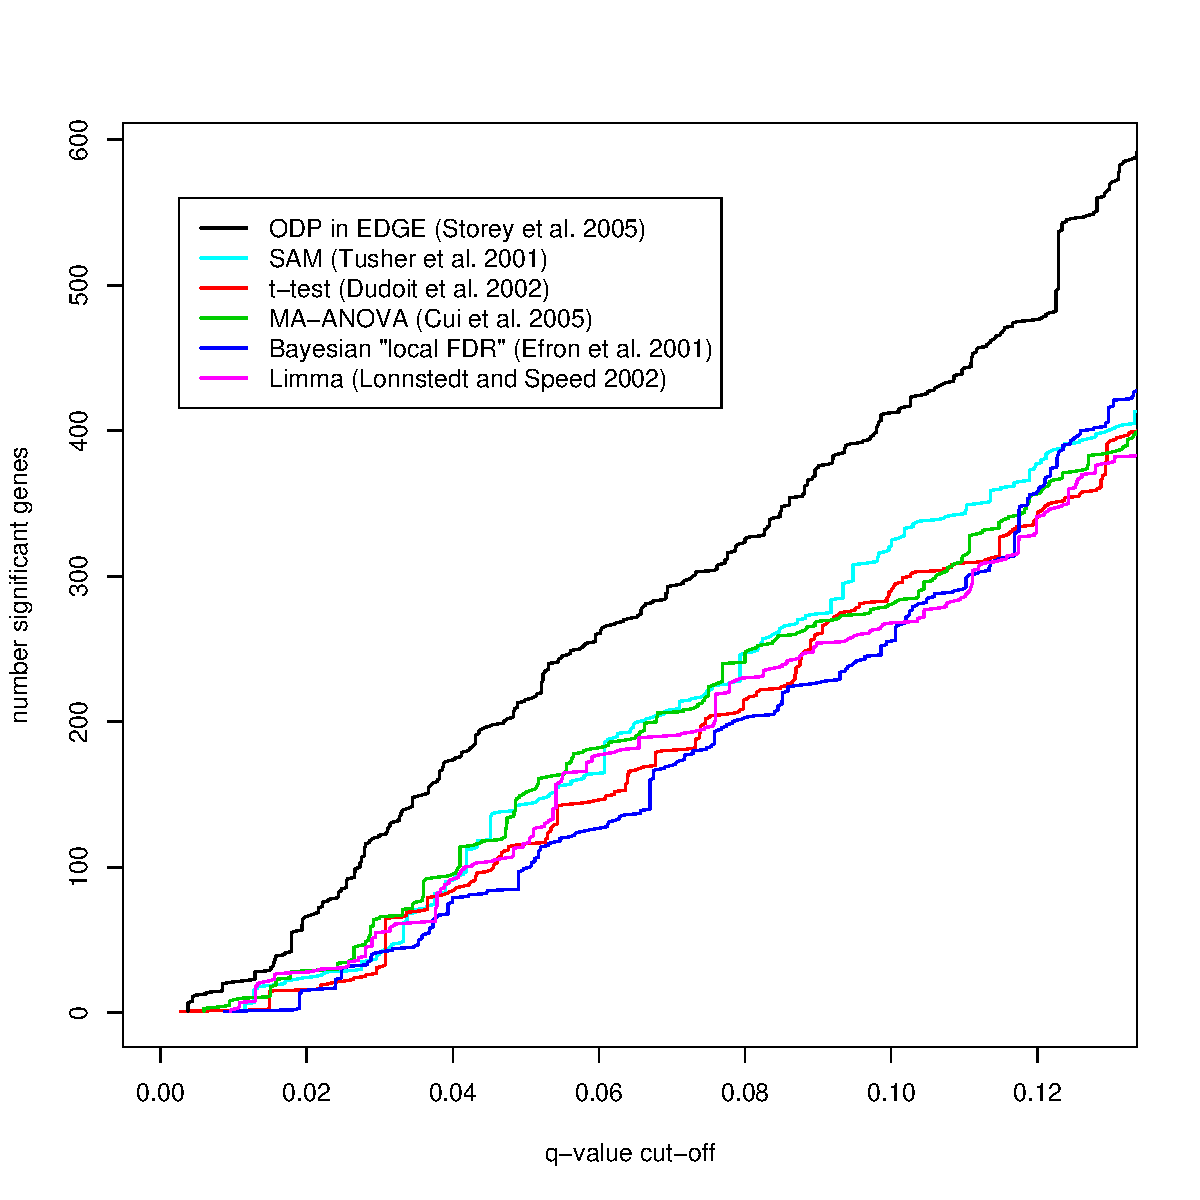
\includegraphics[scale=.50]{edgecomp.pdf}
\caption{Comparison of EDGE to various other leading methods for identifying differential expressed genes in the \cite{hedenfalk:2001} study. Figure is from \cite{leek2005}.}
\label{fig:Comparison}
\end{figure}

\begin{figure}[!htbp]
 \centering
\begin{knitrout}
\definecolor{shadecolor}{rgb}{0.969, 0.969, 0.969}\color{fgcolor}

{\centering \includegraphics[width=\maxwidth]{figure/unnamed-chunk-4-1} 

}



\end{knitrout}
\caption{Plot of the first gene in the {\tt gibson} study.}
\label{fig:gplot}
\end{figure}

\begin{figure}[!htbp]
 \centering
\begin{knitrout}
\definecolor{shadecolor}{rgb}{0.969, 0.969, 0.969}\color{fgcolor}

{\centering \includegraphics[width=\maxwidth]{figure/unnamed-chunk-5-1} 

}



\end{knitrout}
\caption{Plot of the first gene in the {\tt gibson} study after applying the alternative and null model fit. The ``raw'' column is the expression values of the original data.}
\label{fig:gplotFit}
\end{figure}

\begin{figure}[!htbp]
 \centering
\begin{knitrout}
\definecolor{shadecolor}{rgb}{0.969, 0.969, 0.969}\color{fgcolor}\begin{kframe}
\begin{alltt}
\hlkwd{plot}\hlstd{(sig.results)}
\end{alltt}
\end{kframe}

{\centering \includegraphics[width=\maxwidth]{figure/unnamed-chunk-6-1} 

}



\end{knitrout}
\caption{Apply the function {\tt plot} to the slot {\tt qvalueObj}. Function is derived from the {\tt qvalue} package.}
\label{fig:gqvalPlot}
\end{figure}
\begin{figure}[!htbp]
 \centering
\begin{knitrout}
\definecolor{shadecolor}{rgb}{0.969, 0.969, 0.969}\color{fgcolor}\begin{kframe}
\begin{alltt}
\hlkwd{hist}\hlstd{(sig.results)}
\end{alltt}
\end{kframe}

{\centering \includegraphics[width=\maxwidth]{figure/unnamed-chunk-7-1} 

}



\end{knitrout}
\caption{Apply the function {\tt hist} to the slot {\tt qvalueObj}. Function is derived from the {\tt qvalue} package.}
\label{fig:gqvalHist}
\end{figure}



\begin{figure}[!htbp]
 \centering
\begin{knitrout}
\definecolor{shadecolor}{rgb}{0.969, 0.969, 0.969}\color{fgcolor}

{\centering \includegraphics[width=\maxwidth]{figure/unnamed-chunk-8-1} 

}



\end{knitrout}
\caption{Plot of the first gene in the {\tt kidney} study.}
\label{fig:kplot}
\end{figure}


\begin{figure}[!htbp]
 \centering
\begin{knitrout}
\definecolor{shadecolor}{rgb}{0.969, 0.969, 0.969}\color{fgcolor}\begin{kframe}


{\ttfamily\noindent\bfseries\color{errorcolor}{\#\# Error in data.frame(age = age, sex = sex, null.model = fitVals0[1, ], : arguments imply differing number of rows: 72, 46}}

{\ttfamily\noindent\bfseries\color{errorcolor}{\#\# Error: id variables not found in data: age, sex}}

{\ttfamily\noindent\bfseries\color{errorcolor}{\#\# Error: Aesthetics must either be length one, or the same length as the dataProblems:age, sex}}\end{kframe}
\end{knitrout}
\caption{Plot of the first gene in the {\tt gibson} study after applying the alternative and null model fit. The ``raw'' column is the expression values of the original data.}
\label{fig:kplotFit}
\end{figure}

\section*{Acknowledgements}
This software development has been supported in part by funding from the National Institutes of Health and the Office of Naval Research.

\bibliographystyle{plainnat}
\bibliography{edgerefs} 
\end{document}
